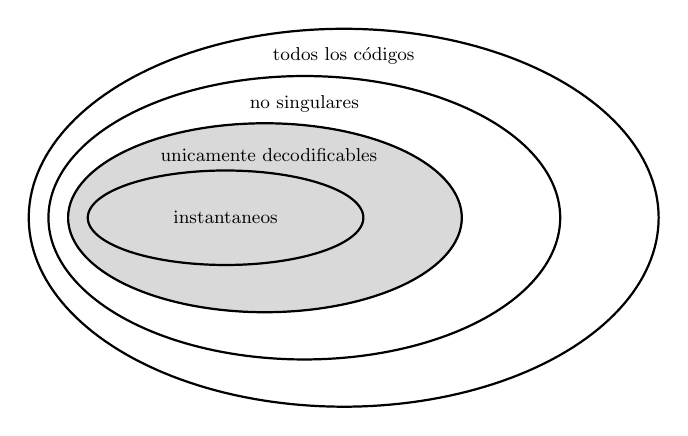
\begin{tikzpicture}
\shorthandoff{>}
\filldraw[fill=gray!30,domain=0:360, samples=200] plot ({2.5*cos(\x)+.5},{1.2*sin(\x)});
%%%%
\draw[thick,domain=0:360, samples=200] plot ({1.75*cos(\x)},{.6*sin(\x)});
\node[scale=.75] at (0,0){\small instantaneos};
%
\draw[thick,domain=0:360, samples=200] plot ({2.5*cos(\x)+.5},{1.2*sin(\x)});
\node[scale=.75] at (.55,.8){\small  unicamente decodificables};
%
\draw[thick,domain=0:360, samples=200] plot ({3.25*cos(\x)+1},{1.8*sin(\x)});
\node[scale=.75] at (1,1.45){\small no singulares};
%
\draw[thick,domain=0:360, samples=200] plot ({4*cos(\x)+1.5},{2.4*sin(\x)});
\node[scale=.75] at (1.5,2.05){\small todos los c\'odigos};
\end{tikzpicture}
